\chapter{Hasil dan Pembahasan}\label{cha:result}

Dalam penelitian ini, analisis statistik deskriptif dilakukan dengan menghitung nilai rata-rata (\textit{mean}) dari setiap item pada skala kuesioner untuk memperoleh pemahaman mengenai persepsi mahasiswa terhadap kualitas antarmuka platform \gls{digilib} IIB Darmajaya. Proses analisis ini menggunakan \textit{toolkit} \gls{ueq} berbasis Microsoft Excel. Data tanggapan dari 17 responden diolah secara sistematis berdasarkan enam dimensi utama \gls{ueq}, yaitu \textit{attractiveness}, \textit{perspicuity}, \textit{efficiency}, \textit{dependability}, \textit{stimulation}, dan \textit{novelty}.

Rangkuman dari hasil penilaian kuantitatif tersebut disajikan secara terstruktur pada Tabel \ref{tab:ueq_mean} di bawah ini, yang memberikan gambaran umum mengenai kecenderungan persepsi pengguna terhadap pengalaman penggunaan sistem.

\begin{table}[htbp]
\centering
\caption{Hasil Rata-Rata Skala UEQ Digilib IIB Darmajaya}
\label{tab:ueq_mean}
\begin{tabular}{|l|c|l|}
\hline
\textbf{Skala Penilaian} & \textbf{Nilai Rata-Rata} & \textbf{Kategori Benchmark} \\ \hline
Attractiveness (Daya Tarik) & 1,01 & Below Average \\ \hline
Perspicuity (Kejelasan) & 1,02 & Below Average \\ \hline
Efficiency (Efisiensi) & 1,13 & Above Average \\ \hline
Dependability (Ketepatan) & 0,89 & Below Average \\ \hline
Stimulation (Stimulasi) & 1,04 & Above Average \\ \hline
Novelty (Kebaruan) & 1,00 & Above Average \\ \hline
\end{tabular}
\end{table}

\begin{figure}[htbp]
\centering
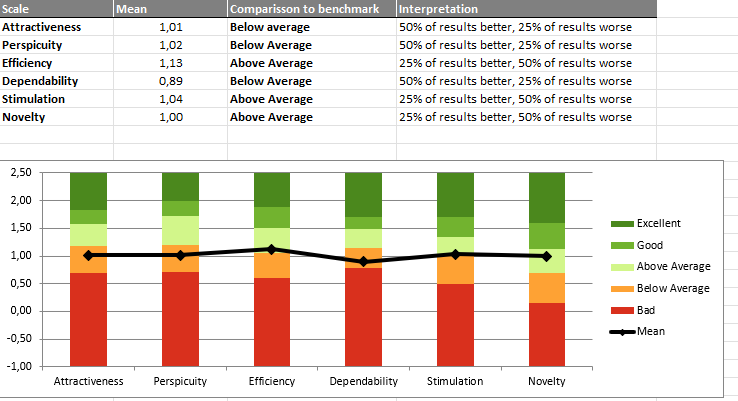
\includegraphics[width=0.8\textwidth]{img/ueq_benchmark.png}
\caption{Hasil Komparasi Benchmark UEQ}
\label{fig:ueq_benchmark}
\end{figure}

Tujuan komparasi data \textit{benchmark} ini adalah untuk mengevaluasi kualitas pengalaman pengguna platform \gls{digilib} IIB Darmajaya berdasarkan standar global yang berisi komparasi dari 21.175 responden terhadap 468 studi produk perangkat lunak (seperti aplikasi bisnis, halaman web, dan jejaring sosial). Hasil perbandingan ini disajikan pada Tabel \ref{tab:ueq_benchmark}.

\begin{table}[htbp]
\centering
\caption{Hasil Komparasi Benchmark UEQ}
\label{tab:ueq_benchmark}
\begin{tabular}{|p{4.5cm}|c|l|p{6cm}|}
\hline
\textbf{Skala (Scale)} & \textbf{Nilai Rata-Rata (Mean)} & \textbf{Kategori Benchmark} & \textbf{Interpretasi} \\ \hline
Daya Tarik (\textit{Attractiveness}) & 1,01 & Below Average & 50\% produk lain lebih baik, 25\% lebih buruk \\ \hline
Kejelasan (\textit{Perspicuity}) & 1,02 & Below Average & 50\% produk lain lebih baik, 25\% lebih buruk \\ \hline
Efisiensi (\textit{Efficiency}) & 1,13 & Above Average & 25\% produk lain lebih baik, 50\% lebih buruk \\ \hline
Ketepatan (\textit{Dependability}) & 0,89 & Below Average & 50\% produk lain lebih baik, 25\% lebih buruk \\ \hline
Stimulasi (\textit{Stimulation}) & 1,04 & Above Average & 25\% produk lain lebih baik, 50\% lebih buruk \\ \hline
Kebaruan (\textit{Novelty}) & 1,00 & Above Average & 25\% produk lain lebih baik, 50\% lebih buruk \\ \hline
\end{tabular}
\end{table}

Berdasarkan Tabel \ref{tab:ueq_benchmark} dan evaluasi \textit{benchmark} di atas, persepsi pengguna terhadap daya tarik (\textit{attractiveness}) berada pada kategori \textit{below average}, menandakan desain antarmuka \gls{digilib} dirasa belum cukup menarik secara visual, di mana 50\% produk sejenis di pasaran memiliki nilai yang lebih baik. Dimensi kejelasan (\textit{perspicuity}) dan ketepatan (\textit{dependability}) juga termasuk dalam kategori \textit{below average}. Hal ini mencerminkan bahwa pengguna masih mengalami kebingungan dalam menavigasi struktur antarmuka serta kurangnya kepercayaan terhadap keandalan sistem saat memproses pencarian atau pemuatan dokumen.

Sementara itu, efisiensi (\textit{efficiency}) dinilai \textit{above average} (di atas rata-rata), menunjukkan bahwa sistem dapat memfasilitasi pengguna untuk menyelesaikan tugas pencarian dengan waktu yang cukup efisien. Dimensi stimulasi (\textit{stimulation}) dan kebaruan (\textit{novelty}) juga berada pada kategori \textit{above average}, mengindikasikan bahwa \gls{digilib} ini secara fungsional dinilai memiliki konsep yang mendukung, inovatif, dan relevan dengan kebutuhan, meskipun eksekusi desain interaksinya masih memunculkan hambatan pragmatis.

\section{Hasil Wawancara}
Untuk memvalidasi dan melengkapi data kuantitatif \gls{ueq}, dilakukan wawancara mendalam dengan perwakilan mahasiswa sebagai pengguna \gls{digilib} IIB Darmajaya. Berdasarkan hasil wawancara, ditemukan beberapa keluhan spesifik yang berbanding lurus dengan rendahnya nilai \textit{dependability} dan \textit{perspicuity}.

Mayoritas narasumber mengeluhkan tata letak (\textit{layout}) halaman pencarian yang terlalu padat, kaku, dan tidak mengelompokkan kategori koleksi referensi secara jelas. Selain itu, sistem filter pencarian dinilai kurang presisi (\textit{dependability} rendah), di mana kata kunci yang dimasukkan pengguna seringkali menampilkan hasil dokumen yang tidak relevan. Dari segi \textit{attractiveness}, pengguna menilai antarmuka terkesan monoton dan tidak diperbarui sesuai standar \gls{ui} modern. Meskipun kecepatan respons sistem dinilai baik, alur navigasi yang berbelit-belit memaksa mahasiswa harus melalui terlalu banyak tahapan (\textit{clicks}) hanya untuk menemukan dan mengunduh satu dokumen yang dituju.

\section{Pembahasan}
Berdasarkan hasil pengujian, evaluasi antarmuka pada aplikasi \gls{digilib} IIB Darmajaya menunjukkan bahwa pengalaman pengguna secara menyeluruh masih jauh dari titik optimal. Dominasi kategori penilaian di bawah rata-rata (\textit{below average}) pada aspek pragmatis maupun visual---terutama \textit{Dependability} (0,89), \textit{Attractiveness} (1,01), dan \textit{Perspicuity} (1,02)---menjadi indikator kuat bahwa sistem saat ini masih memberikan beban kognitif (\textit{cognitive load}) yang tinggi bagi pengguna. Hal ini menuntut adanya perombakan desain yang harus berfokus pada perbaikan arsitektur informasi, penyederhanaan alur interaksi (\textit{user flow}), serta perbaikan algoritma penyaringan data agar hasil pencarian literatur menjadi lebih akurat.

Meskipun aspek \textit{efficiency}, \textit{stimulation}, dan \textit{novelty} menunjukkan hasil \textit{above average}, angka tersebut masih merujuk pada rentang evaluasi yang netral menuju positif ringan (skor 1,00 - 1,13). Angka ini belum mencapai rentang optimal (kategori \textit{good} atau \textit{excellent}). Temuan penelitian ini menegaskan bahwa untuk meningkatkan utilitas dan intensitas penggunaan \gls{digilib} sebagai sumber utama referensi akademik mahasiswa, pengelola sistem tidak cukup hanya mempertahankan stabilitas \textit{back-end} atau server. Diperlukan komitmen untuk menerapkan pendekatan \textit{User-Centered Design} (UCD) pada \textit{front-end} aplikasi agar ekosistem digital kampus menjadi lebih ramah pengguna, intuitif, dan secara langsung berdampak positif terhadap kepuasan layanan sivitas akademika.